%%% The ``\documentclass'' command has one parameter, based on the kind of
%%% document you are preparing.
%%%
%%% [annual] - Technical paper accepted for presentation at the ACM SIGGRAPH 
%%%   or SIGGRAPH Asia annual conference.
%%% [sponsored] - Short or full-length technical paper accepted for 
%%%   presentation at an event sponsored by ACM SIGGRAPH
%%%   (but not the annual conference Technical Papers program).
%%% [abstract] - A one-page abstract of your accepted content
%%%   (Technical Sketches, Posters, Emerging Technologies, etc.). 
%%%   Content greater than one page in length should use the "[sponsored]"
%%%   parameter.
%%% [preprint] - A preprint version of your final content.
%%% [review] - A technical paper submitted for review. Includes line
%%%   numbers and anonymization of author and affiliation information.

\documentclass[annual]{acmsiggraph}

%%% If you are submitting your paper to one of our annual conferences - the 
%%% ACM SIGGRAPH conference held in North America, or the SIGGRAPH Asia 
%%% conference held in Southeast Asia - there are several commands you should 
%%% consider using in the preparation of your document.

%%% 1. ``\TOGonlineID''
%%% When you submit your paper for review, please use the ``\TOGonlineID''
%%% command to include the online ID value assigned to your paper by the
%%% submission management system. Replace '45678' with the value you were
%%% assigned.

\TOGonlineid{45678}

%%% 2. ``\TOGvolume'' and ``\TOGnumber''
%%% If you are preparing a preprint of your accepted paper, and your paper
%%% will be published in an issue of the ACM ``Transactions on Graphics''
%%% journal, replace the ``0'' values in the commands below with the correct
%%% volume and number values for that issue - you'll get them before your
%%% final paper is due.

\TOGvolume{0}
\TOGnumber{0}

%%% 3. ``TOGarticleDOI''
%%% The ``TOGarticleDOI'' command accepts the DOI information provided to you
%%% during production, and which makes up the URLs which identifies the ACM
%%% article page and direct PDF link in the ACM Digital Library.
%%% Replace ``1111111.2222222'' with the values you are given.

\TOGarticleDOI{1111111.2222222}

%%% 4. ``\TOGprojectURL'', ``\TOGvideoURL'', ``\TOGdataURL'', ``\TOGcodeURL''
%%% If you would like to include links to personal repositories for auxiliary
%%% material related your research contribution, you may use one or more of
%%% these commands to define an appropriate URL. The ``\TOGlinkslist'' command
%%% found just before the first section of your document will add hyperlinked
%%% icons to your document, in addition to hyperlinked icons which point to
%%% the ACM Digital Library article page and the ACM Digital Library-held PDF.

\TOGprojectURL{}
\TOGvideoURL{}
\TOGdataURL{}
\TOGcodeURL{}

%%% Replace ``PAPER TEMPLATE TITLE'' with the title of your paper or abstract.

\title{PerVERT: Performance Visualization and Error Remediation Toolkit}

%%% The ``\author{}'' command takes the names and affiliations of each of the
%%% authors of your paper or abstract. The ``\thanks{}'' command takes the
%%% contact information for each author.
%%% For multiple authors, separate each author's information by the ``\and''
%%% command.

\author{Niels Joubert\thanks{e-mail:njoubert@cs.stanford.edu}\\ Stanford University %
\and Eric Schkufza\thanks{e-mail:eschkufz@cs.stanford.edu}\\ Stanford University}

%%% The ``pdfauthor'' command accepts the authors of the work,
%%% comma-delimited, and adds this information to the PDF metadata.

\pdfauthor{Niels Joubert, Eric Schkufza}

%%% Keywords that describe your work. The ``\keywordlist'' command will print
%%% them out.

\keywords{performance visualization, JIT, compiler, instrumentation}

%%% The ``\begin{document}'' command is the start of the document.

%%% If you have user-defined macros, you may include them here.

% example of a user-defined macro called ``remark.''
% \newcommand{\remark}[1]{\textcolor{red}{#1}}

\begin{document}

%%% A ``teaser'' image appears under the title and affiliation information,
%%% horizontally centered, and above the two columns of text. This is OPTIONAL.
%%% If you choose to have a ``teaser'' image, it needs to be placed between
%%% ``\begin{document}'' and ``\maketitle.''

\teaser{
   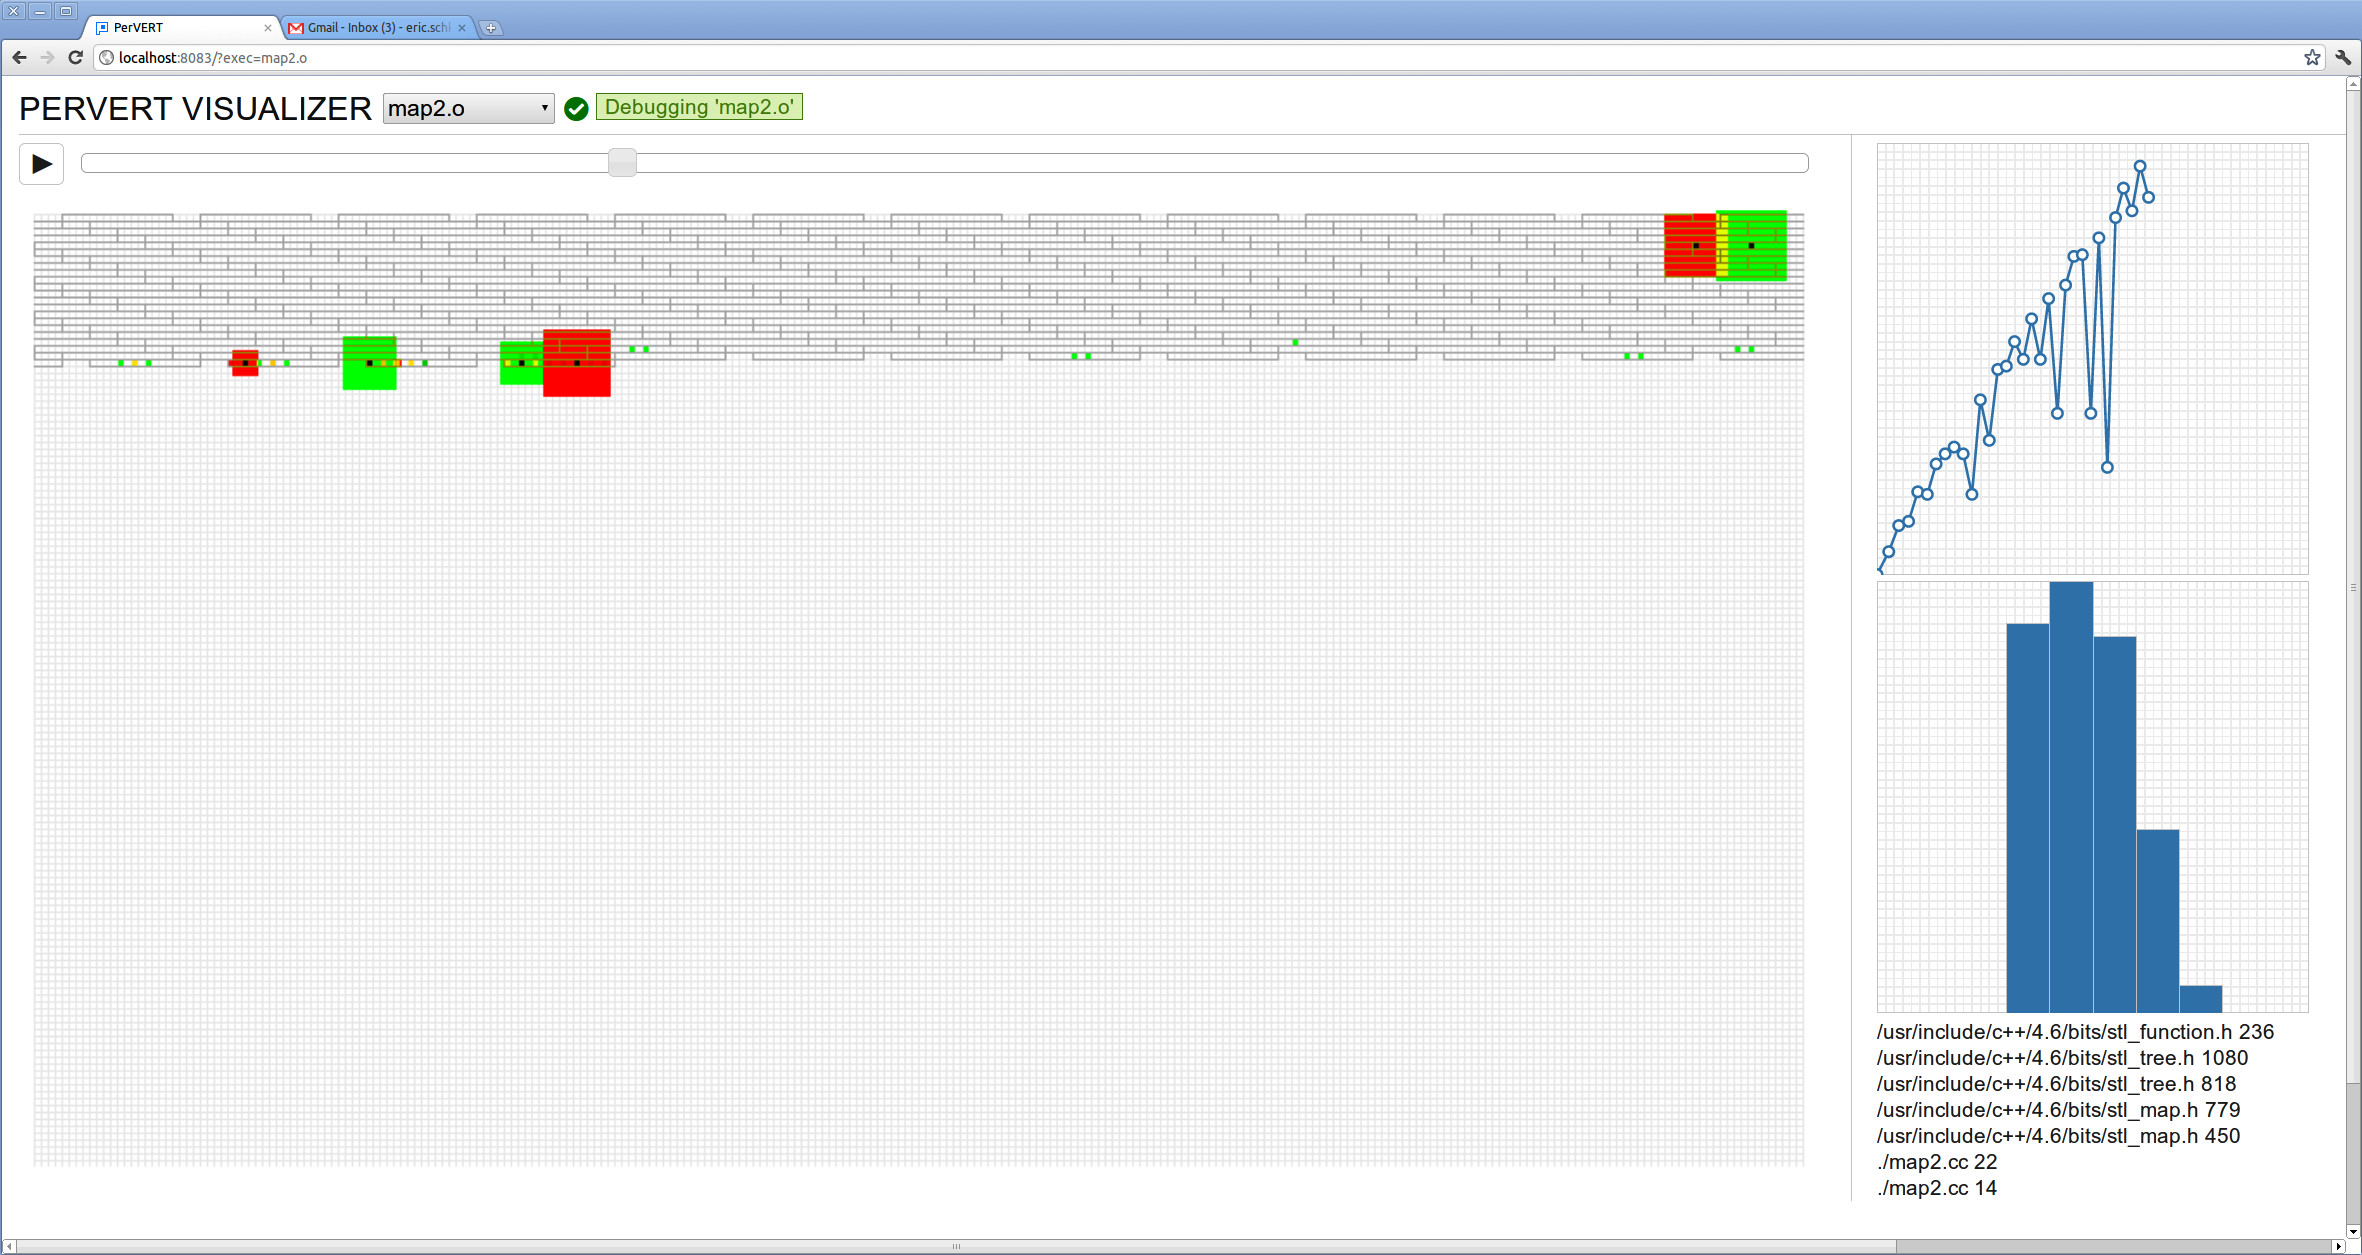
\includegraphics[height=3in]{images/pervert.png}
   \caption{The PerVERT tool}
}

%%% The ``\maketitle'' command must appear after ``\begin{document}'' and,
%%% if you have one, after the definition of your ``teaser'' image, and
%%% before the first ``\section'' command.

\maketitle

%%% Your paper's abstract goes in its own section.

\begin{abstract}

Performance tuning is an important step in the development large software systems. 
Examples include web-servers which routinely handle thousands of simultaneous content requests, 
  and petaflop supercomputers which perform physical simulations that span tens of thousands of cpu cores. 
As improvements in clock frequency slow and hardware trends continue towards increased parallelism, 
  the runtime performance of these and similar systems will become ever more a function of memory efficiency. 
Unfortunately, the ability to effectively reason about this phenomenon using existing tools such as 
  valgrind \cite{Nethercote:2007:VFH:1250734.1250746}, 
  gprof \cite{Graham:2004:GCG:989393.989401}, 
  or gdb \cite{stallman1991using}, 
  through a text-based interface, is limited, and tedious at best.

We present PerVERT, an instrumentation framework for logging a process's virtual memory traffic and a visualization suite for reasoning about common memory performance bugs: 
  Are memory accesses organized coherently in both spatial and temporal dimensions? 
  To what extent do these patterns differ based on program inputs or changes in source code?
\end{abstract}

%%% ACM Computing Review (CR) categories.
%%% See <http://www.acm.org/class/1998/> for details.
%%% The ``\CRcat'' command takes four arguments.


%%% The ``\keywordlist'' command prints out the keywords.

\keywordlist

%%% The ``\TOGlinkslist'' command will insert hyperlinked icon(s) to your
%%% paper. This includes, at a minimum, hyperlinked icons to the ACM article
%%% page and the ACM Digital Library-held PDF. If you added URLs to
%%% ``\TOGprojectURL'' or the other, similar commands, they will be added to
%%% the list of icons.
%%% Note: this functionality only works for annual-conference papers.

\TOGlinkslist

%%% The ``\copyrightspace'' command 
%%% Do not remove this command.

\copyrightspace

%%% This is the first section of the body of your paper.

\section{Introduction}
  
%   \begin{itemize}
%   \item Many people care about having high performance codes, which need to be as fast as possible. 
%   \item Performance means minimizing time -- interested in viewing events over time.
%   \item Performance is often a function of memory efficiency because memory is so much slower than compute.
%   \item Performance is considered a "black art" and very difficult to get right, since it's a secondary effect of code.
% 
%   \item Most debugging tools are built for correctness, which is a property of the computations done on the program's state. This leads to a control-flow-centric view of the world, where the transformations your code does is inspected.
%  \item Performance is a more global property depending on the actual data usage, thus a data-centric view is a more natural fit.
%  \item Performance is also a global property since data layout directly affects access patterns, which is state hidden from the code being written.
%  \item Even simple code can cause incredibly complicated access patterns and consume lots of data.
%  \item Thus, we want to use a visual approach to aggregate lots of data, and do this in a data-centric view that directly shows how memory is accessed.
%  \end{itemize}
  
  Users and developers alike care about the performance of computer programs. It's commonly understood that good performance can often be the distinguishing factor in the usability of a code. This is especially true is the scientific and financial simulation communities, where long-running codes have to share computing power on clusters of machines.
  
  As computers become faster and processor count increase, performance becomes more and more a function of memory efficiency. Memory speeds are not increasing at the same rate as computing power, and the cost of communicating data by touching memory is becoming the primary factor in degrading performance. For this reason, tuning the memory access patterns of a code is the primary way of increasing performance of the same algorithm. This is an important distinguishment - given the same correct code, performance is increased by using smarter datastructures with smarter access patterns to them.
  
  Performance tuning is still considered a ``black art'' due to the opaqueness of performance: while code directly expresses computation, the time it takes for a computation is a second order effect of the code. This is especially true for accessing memory, where the memory hierarchy is completely invisible to the user.
  
  Improving the performance of code means minimizing the time it takes to compute a result. For this reason, people measure performance in terms of events per amount of time. To be able to improve the performance of code, we must get insight into this currently-opaque operations of memory accesses, and understand how they relate to the code.
  
  Most debugging tools are built to help with the correctness of code, which is a property of the computations done on the program's state. This naturally leads to a control-flow-centric view of the program: what is the transformations and are they performing the correct behavior on their input data? Debugging works well when the tool breaks the program into small parts that can be understood and checked for correctness locally.
  
  Performance does not nicely follow this model, since performance is a global phenomenon - the layout of data directly affects the accesses performed by other parts of the code. Performance concerns also cuts through the normal barriers between third party libraries and your own code. It's thus important to understand the memory accesses of your program using a \emph{data-centric} approach: looking at memory accesses as events happening on data regardless of where it comes from. This needs to happen both on a global level to support understanding these concerns and on a local events level to tie events back to the code performing them, so that the programmer can change their code.
    
  The massive amounts of data, chaotic global changes in this dataset, and the natural spatial layout of a physical memory system leads naturally to a visual representation of this data. To that end, this paper presents a visual performance tuning tool that presents global structure, local events, and aggregate statistics of a code's memory performance, with the intent of helping the user identify problems, find solutions, and implement these solutions. 
  
  The remainder of this paper is structured as follows. In section \ref{ch_dg} we present goals for the design and use of this system. In section \ref{ch_d} we present the visual and interaction design of this system, and how we anticipate developers using this system. In section \ref{ch_i} we show the inner workings of this system and how we supported our design while meeting our design goals. Lastly we discuss related and future work.
    
\section{Design Goals}\label{ch_dg}

  \subsection{Binary Instrumentation}
  %\begin{itemize}
  %\item At what level do we work? Performance depends on everything happening in your program, including the parts you have no insight into - libraries and system calls/
  %\item It lowers the barrier to performance tuning when the same toolset can inform you about your code and the libraries you are using.
  %\item Workin at a binary level provides transparency through everything an app uses, including system and third party libs.
  %\end{itemize}

  Performance is an aggregate property of a software system.
  It depends on every layer of code which is executed, including those that the user often has no insight into:
    libraries and system calls.
  This barrier to optimization could be substantially lowered by a toolset that could instrument both.
  Additionally, by instrumenting code at the binary level, the resulting transparency can extent not only through
    all layers of the code, but through to the choice of programming language as well.

  \subsection{Remote Analysis}
  %\begin{itemize}
  %  \item development vs production machines look very different
  %  \item often need to perftune remotely
  %  \item ideal to ship as little data from back-end to front-end, so analysis runs on back-end and vis runs on front-end.
  %\end{itemize}

  For many high performance software systems, development and production environments are completely distinct.
  Development often takes place remotely, and code is run on exotic hardware that does not even support a graphical environment.
  Running analysis directly on the backend and shipping the results to a thin visualization client would enable 
    the user to debug performance in the same environment that he develops in.
  Additionally, divorcing data analysis from visualization would allow multiple developers to inspect the same performance
    log simultaneously.

  \subsection{On-Demand Analysis}
  %\begin{itemize}
  %  \item massive amounts of data, aggregated into many different ways, with multiple views of this data
  %  \item cannot do all analysis ahead of time
  %  \item do no want to do unneeded analysis
  %  \item thus we build a tool that can do analysis on-the-gly
  %\end{itemize}
   
  High performance software systems generate enormous amounts of profiling data.
  Aggregating and visualizing that data statically would be intractable, 
    both in terms of computational effor and storage requirement.
  This complexity could be overcome both through caching and a combination of statically computing only what can
    be stored efficiently and computing all other analyses on demand.

\section{Design}\label{ch_d}
  \subsection{Memory Map}

  	\begin{figure}[t]
  		\centering
      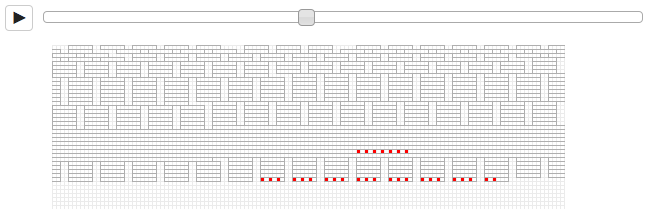
\includegraphics[scale=0.40]{images/memmap.png}
  		\caption{Memory Map display showing global structure of memory sized to the width of cache lines, with local events marked by color as reads (green) or writes (red).}
      \label{fig:memmap}
  	\end{figure}
  
  We want to support understanding memory accesses in a global sense. To that end, we present a program's virtual memory space as a spatial layout of memory. Memory addresses are physically arranged in caches, where a cache line contains on the order of hundreds of individual memory locations, and subsequent accesses within a cache line have different performance characteristics than accesses that cross cache lines. This physical property of the system gives a clue to the correct visual design of the memory layout - by directly representing all of memory segmented into cache lines, there's a good impedance match between memory events of a program and the physical accesses that occur. We thus present the entire memory space as a grid of memory locations, where each row corresponds to a single cache line.
  
  In figure ref{fig:memmap} we show this grid. We now want to visualize memory events - actions a program performs that impacts the memory system. As we previously stated, performance tuning attempts to minimize the amount of time a code takes to run, and memory events also happen over time. This leads us to display events over time using animation. 
  
  We visualize four different types of events: memory region allocation, memory region deallocation, reads and writes.
  
  Region allocation and deallocation affects the structure of memory, thus we present it using structural visual cues. Allocation regions are shown by highlighting those areas of the memory grid, and deallocations causes these highlights to go away.
  
  Reads and Writes causes memory traffic to happen to a certain address. We represent this visually by highlighting the grid cell corresponding to the memory address, in red for writes and in green for reads. By distinguishing colors, it's possible to visually see copies between locations happening, which is a strong indicator to optimize the performance of code by doing zero copies.
    
  Memory performance is at a maximum when accesses are both temporally and spatially local. We want to provide a visual cue to help the user judge the spatial locality of memory access over a period of time. To support this, we show a short history of memory accesses by highlighting not just the current but the last 50 cells accessed. By showing history trails we provide a visual cue to how chaotic memory accesses are, so the user can visually judge whether accesses are happening primarily in the same cache line or jumping between cache lines. This has a direct influence on the performance of their code, so it highlights problems with code as well as hinting at possible solutions.
  
  Given this framework we have to somehow highlight the current access and provide a strong visual cue for what's currently happening. With no highlighting of the current event, the currently described display is difficult to follow since accesses happen on individual cells of a pixel grid. By enlarging the grid slightly we make it easier to see individual accesses - a fair tradeoff against seeing less of total memory at one time.
  
    	\begin{figure}[t]
  		\centering
      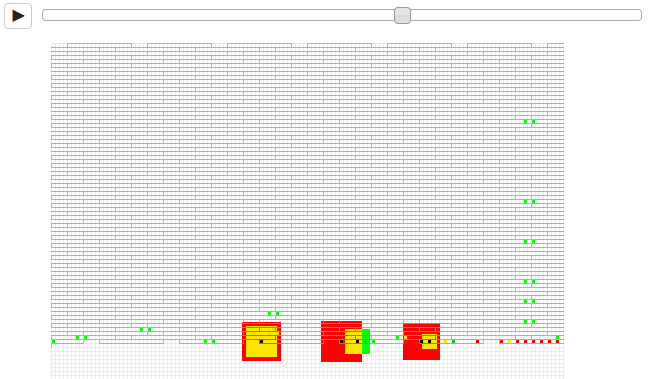
\includegraphics[scale=0.40]{images/fireworks.png}
  		\caption{Fireworks with alpha blending shown on memory map, highlighting memory events as they occur and overlap}
      \label{fig:fireworks}
  	\end{figure}

  
  We highlight current accesses by using a technique we call ``fireworks'' - highlighting a large block of memory centered on the current access, and animating this access to zoom down onto the cell it touches, shown in figure \ref{fig:fireworks}. This gives a very strong visual cue to the local changes occuring without sacrificing our view of global structure.
  
  A single memory location can be accessed multiple times using both reads and writes following one another. We want to visually distinguish points in our history trail that have many accesses to them versus those that have a single access. Similarly, we want to visually distinguish fireworks that happen on top of one another depending on the type of accesses - reads or writes. We use a technique called ``alpha blending'' to change the color of a cell as different types of accesses happen on it. For example, a cell that is accessed by alternating reads and writes now becomes fireworks of greens and reds, and with their overlap colored yellow. In the same way, a cell that is accessed by mostly reading and sometimes writing will be colored mostly green (reads) with a small amount of red (writes). This display gives visual cues to the access patterns of an individual cell in the same way that history trails gives access patterns to different memory cells.
  
  \subsubsection{Interaction}
    The first level of interaction with this memory map is through watching an animation play back. The set of visual cues we've described leads to interesting events being very obvious, and begging further inspection. We provide a time slider to show progress over time and interacting with the current point in time.
    
      \begin{figure}[t]
  		\centering
      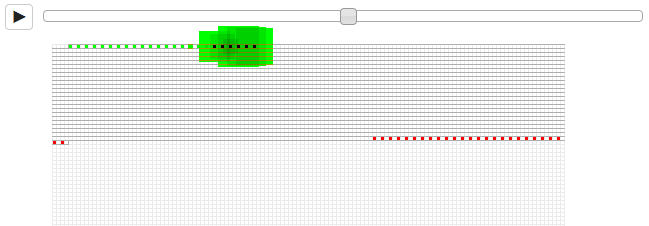
\includegraphics[scale=0.40]{images/array_fireworks.png}
  		\caption{Interaction happens primarily through the play/pause button, stepping the code with the keyboard, or scrubbing the time slider.}
      \label{fig:fireworks}
  	\end{figure}

    
    We provide controls to pause the animation, and scrub through time or step forwards and backwards in time. By scrubbing an event you can roll up into a higher level view of quickly moving through accesses to compare memory behavior over larger chunks of time. If a locally interesting event happens, stepping over it gives time to mentally reason about the behavior.
    
    This implementation of the memory map is primarily focused on identifying problems. Once a problem area has been identified, PerVERT can be paused at this point in time program's execution, and the aggregate statistics presented next can be inspected for this event.
  
  
%     \begin{itemize}
%       \item PICTURE OF MEMMAP
%       \item Performance is a global property 
%       \item Therefore: Grid-based representation of the virtual address space.
%       \item Physical cache structure has a huge impact on performance -- represented directly in the visualization.    
%       \item Therefore: Rows correspond to cache lines.
%       \item Memory events happen over time: Visualize as animation
%       \item One memory location can be used for many different malloc'd regions, therefore not a static snapshot over all time
%       \item Four types of events: mallocs, frees, reads, writes
%       \item Visual cues for malloced regions - heavy outlines for those cells
%       \item Visual cues for reads and writes - highlight memory accesses by coloring cells.
%       \item Visual history of recent accesses - s
%       \item Fireworks to highlight local changes.
%       \item Alpha blending gives cues to access patterns: R, W, mix
%    \end{itemize}
% 
% Interaction:
%    \begin{itemize}   
%       \item Watching the animation shows visual queues leads to interesting events being very obvious, begs further inspection.
%       \item Pausing, Stepping fwd and back allows deeper inspection of interaction between temporally local events.
%       \item Scrubbing and Jumping through all time quickly allows for quick memory access comparisons at different points in time.
%       \item This implementation of the memory map aids in identifying problem areas.
%     \end{itemize}
  
  \subsection{Code Context}
    %\begin{itemize}
    %  \item PICTURE OF CODE CONTEXT
    %  \item Every event was caused by an instruction, and thus has an associated context: the stacktrace that caused it.
    %  \item We wish to find the code that caused this event.
    %  \item We display entire stacktrace, incl. user and library code
    %\end{itemize}

  	\begin{figure}[t]
  		\centering
      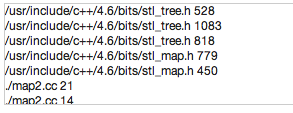
\includegraphics[scale=0.55]{images/context.png}
  		\caption{Code Context window showing the stacktrace of an event.}
      \label{fig:context}
  	\end{figure}


    Every event in a memory trace is caused by a single instruction with an associated context: the stacktrace which produced it.
    This information is extremely valuable, and shown in figure \ref{fig:context}.
    It allows the user to associate behavior in the memory map visualization (both good and bad) 
      with the source code that produced it.
    Accordingly, we display stack traces for every frame in the memory map visualization, 
      including both user code and library code.
  
  \subsection{Context Access Patterns}
    %\begin{itemize}
    %  \item PICTURE OF TWO ACCESS PATTERNS
    %  \item Once a piece of code is identified, the user can further inspect the behavior of this context.
    %  \item For a given context we can drill down into the memory access patterns it causes
    %  \item It's common to reason about the stride of a context - understanding the distances between accesses it causes.
    %  \item Hitogramming strides gives insight into the caching behaviour of this code.
    %  \item We also want to distinguish whether a context is always problematic or only in this instance, histograms does not show time.
    %  \item A complementary view to show access pattern of context over all time
    %  \item Inspecting a combination of these two views gives an overall insight into the caching behavior of the code and suggests approaches to fix it - change the stride or change the data layout.
    %\end{itemize}

  	\begin{figure}[t]
  		\centering
      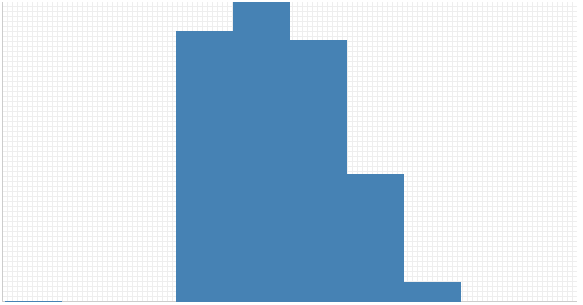
\includegraphics[scale=0.40]{images/histo.png}
  		\caption{Histogram showing memory access strides}
      \label{fig:system}
  	\end{figure}


    Once a stack context is identified as problematic, a user may wish to further inspect its behavior.
    One particular method for doing so, which is often useful, is to examine its stride:
      the address distance between the accesses that it produces.
    PerVERT provides two complementary visualizations for doing so.

    A histogram view aggregates strides for a context over the entire run of the program.
    This view provides insight into its caching behavior.
    Values are binned in powers of 2 bytes up to the length of a cache line.
    Contexts that spend the majority of their time taking large strides, likely often result in cache misses.
    
    \begin{figure}[t]
  		\centering
      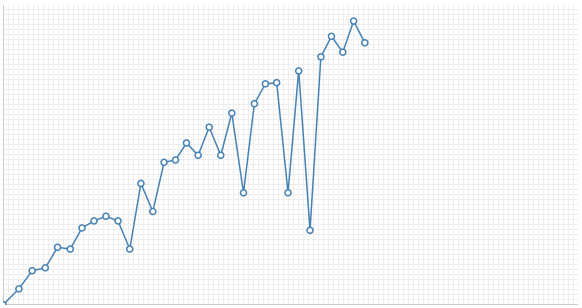
\includegraphics[scale=0.40]{images/line.png}
  		\caption{Line graph showing memory accesses for a context over all time}
      \label{fig:system}
  	\end{figure}

    
    A line graph view shows strides over all time.
    This view allows the user to distinguish between a context which is consistently problematic, 
      and one that exhibits poor striding behavior over only a small segment of a program's execution.

    Inspecting both these views gives an overall insight into the overall caching behavior of a program 
      and suggests an approach for addressing non-performant code.
    Either change the striding pattern of the code, or modify its data layout.

\section{Implementation}\label{ch_i}
  %\begin{itemize}
  %  \item SYSTEM DIAGRAM
  %  \item Built up from three parts -- described below
  %\end{itemize}

	\begin{figure}[t]
		\centering
    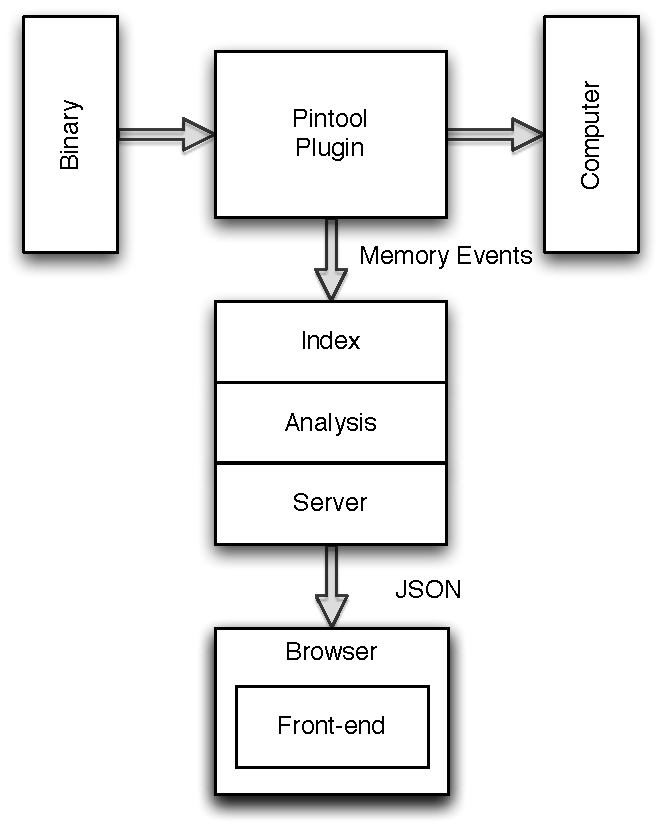
\includegraphics[scale=0.55]{images/SystemDiag.pdf}
		\caption{The implementation of PerVERT.}
    \label{fig:system}
	\end{figure}

  PerVERT consists of five separate components as suggested by Figure \ref{fig:system}:
    a binary instrumentation tool for recording memory traces from program executions,
    an analysis engine for indexing those traces,
    a backend data server for performing on demand analyses on top of those indices,
    an HTTP JSON server for serving that data,
    and a front end for visualizing that data to the user.
  These components are described in detail below.  

  \subsection{Binary Instrumentation}
%    \begin{itemize}
%      \item What it is: Pintool plugin
%      \item Programming language agnostic instrumentation tool.
%      \item Works on code written in any language that compiles to x86 binary.
%      \item Produces memory trace
%      \item Intercept X86 to find read/write instructions
%      \item Intercept function calls to find malloc/free
%      \item Save as trace file
%    \end{itemize}

    The binary instrumentation component of the PerVERT pipeline is a plugin for Intel's pintool \cite{Luk:2005:PBC:1065010.1065034}:
      a language agnostic JIT instrumentation framework for X86 object files.
    Because of this, PerVERT can be run object code irrespective of its original source language.

    PerVERT produces a memory trace by intercepting each of a program's instructions, just before they are executed.
    Reads and writes are found by extracting the arguments from opcodes which are known to touch memory,
      wheras calls to malloc and free are found by identifying jumps to addresses which correspond to those functions
      in the symbol table.
    Reads and writes to addresses that do not appear within malloc'ed regions of the heap are ignored.  
    The resulting trace is written out to a file, and each element is annotated with the stack context in which it occurred.  

  \subsection{Backend}
    %\begin{itemize}
    %  \item System is designed to handle massive amounts of data.
    %  \item Static index built over that data.
    %  \item On demand analysis done in response to user interaction.
    %  \item To optimize this, we unify analysis of and interface to data.
    %\end{itemize}

    The PerVERT backend is designed to handle massive amounts of data.
    It is no uncommon for even a modestly sized program to generate in excess of one million memory events.
    The PerVERT backend builds a static index over each memory trace that it produces, 
      and performs on demand analysis when necessary in response to user interactions.
    To minimize the amount of time spent transmitting the resulting data, 
      PerVERT's analysis engine and data server are unified.
    We describe this architecture below.

    \subsubsection{Index}
      %\begin{itemize}
      %  \item What is is: Persistent long running analysis server
      %  \item Read and index trace files (what indices?)
      %  \item Read and index debug symbols from executable (what symbols?)
      %\end{itemize}

      The PerVERT analysis engine is responsible for building static indices over memory traces.
      This includes tracking memory events by type: read, write, malloc, or free,
        as well as by context.
      For any event, the analysis engine records the stack context that produced the event, 
        as well as pointers to all other events produced by that context.       
      The PerVERT analysis engine also indexes a program's debugging symbol library so that it can decode
        hexademical stack traces to lists of file-line pairs.

      % june sandwich -- 
      % niels below

    \subsubsection{Server}
      The analysis engine performs a set of operations whenever a new binary is traced. Once this analysis is complete, the data has to be made available in a form that's quickly transmitted and easily consumed by the front-end. As the user explores a program, some analysis has to happen dynamically, so events on the front-end has to trigger new analyses. Since we want the front-end to be divorced from the analysis engine, so that analysis can happen close to the code while the front-end can run on a different machine, we implement a client-server infrastructure where the data server is contained inside the analysis engine.
      
      The server itself takes the form of a HTTP JSON server. The server publishes a set of paths that returns information to the front-end. Each path is associated with a different type of information, and takes parameters to specify the exact version of the information we're interested in. For example, the memory map publishes a path that computes the set of memory events and regions at a specific point in time for a specific executable. The front-end can thus request exactly and only the information it needs to display to the user, and the back-end does not need to track any state.
      
      The server itself is engineered in the ``Rack''-style\cite{rack} of web servers, where multiple layers of middleware are plugged together to provide a full stack web server written as a set of modules.
      
      The server runs presistently in the background, even between traces of executables. This makes it possible to capture multiple traces of the same executable for future analysis, and capture multiple different executables so that multiple people can use the tool on the same machine.
      
      Since the API is completely stateless, multiple users and view the same program at the same time, and all data transferred can be cached on either side. This allows for complete flexibility in when analysis happen and how data is caches for the most efficient view of the data.
      
          
      % \begin{itemize}
      %   \item HTTP JSON server
      %   \item Serves frontend / presents JSON api
      %   \item Persistently captures all executables so that you can do comparisons between runs.
      %   \item A stateless api so that multiple users can view the same data or one user can close and come back.
      % \end{itemize}

  \subsection{Frontend}
    
    The visualization is built as a HTML5 ajax application. All user interaction initiates asynchronous requests for textual data from the back-end. This information is then rendered as visualizations using a suite of toolkits.
    
    Any communication to the backend is stateless. To support a highly interactive experience, all back-end data is cached. The user can now perform quick comparisons between data by flipping back and forth without having to request data from the back-end. It also lowers the stress on the back-end server.
    
    The memory map requires drawing a large space with custom visualizations. Since performance of this view is critical, we implement it by drawing pixels on a HTML Canvas element. We stack several of these canvas elements to avoid having to redraw all the layers every frame. The alpha-blending of different accesses is implemented as a standard Alpha Compositing algorithm on the pixel level.
    
    Graphs of aggregate statistics are built using D3, and drawn on-demand by events firing from the user's interaction with the time slider, or as time animated. These graphs each fire their own data requests to the caching layer, and can thus easily be swapped out for different displays.
    
  
    % \begin{itemize}
    %   \item Web app: user interaction initiates asynchronous request for textual data - then render as visualizations.
    %   \item Caching layer stores interaction history to minimize backend communication
    %   \item Use canvas to draw memory space / pixel pushing.
    %   \item D3 to draw aggregate statistics
    % \end{itemize}

\section{Example Applications}\label{ch_e}
  % No outline - we never specced this paragraph out

  \subsection{Algorithm}
    To evaluate PerVERT, we built a test suite of algorithmic variants for a same simple routine
      which one would expect to find a scientific computation kernel.
    (1) Create a container of objects on the heap.
    (2) Write values to each of those objects.
    (3) Read values from each of those objects.
    (4) Free the objects and the container.

    The variants differ only in the type of container used.

  \subsection{Variants}
  
  \begin{figure}[t]
		\centering
    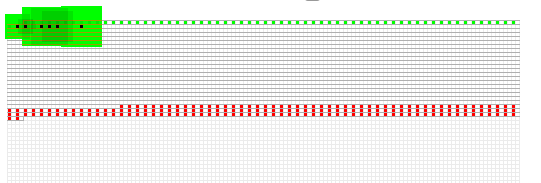
\includegraphics[scale=0.45]{images/example_array.png}
		\caption{C Array example}
    \label{fig:example_array}
	\end{figure}
  
  \subsubsection{C Array}
  For this example we inserted and read a set of integers into and from a C array, shown in figure \ref{fig:example_array}.
  
  In the C++ Array view, the animation reveals two distinct sections of the code's behavior. Initially a linear progression of writes to memory occur as values gets inserted into the array. Once this is complete, a second linear pass over the array reads values back. 

  \subsubsection{C++ STL Vector}
  
  \begin{figure}[t]
		\centering
    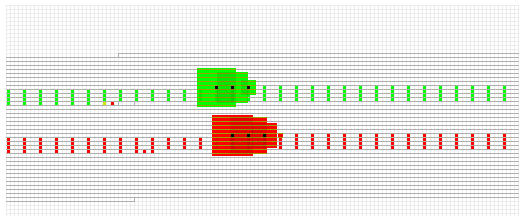
\includegraphics[scale=0.45]{images/example_vector.png}
		\caption{C++ STL vector example}
    \label{fig:example_array}
	\end{figure}
  
  For this example we inserted and read a set of integers into and from a C++ vector, shown in figure \ref{fig:example_vector}.
  
  The vector starts off as a short 4-element array. As values are written to this array, the dynamic resizing of the array and the cost associated with that can immediately be seen: after 4 writes, a new array is allocated and all the previous values are copied to this longer array. This pattern of inserts, followed by enlarge and copy, now makes up the first section of the array. The same behavior of the array's second section can still be seen, where a linear read of the entire final array happens.

  \subsubsection{C++ STL Map}
  
  \begin{figure}[t]
		\centering
    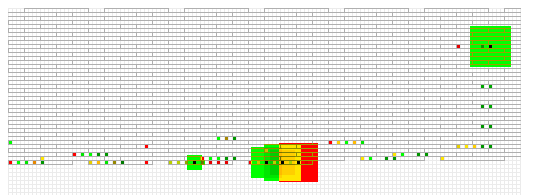
\includegraphics[scale=0.45]{images/example_map.png}
		\caption{C++ STL map example}
    \label{fig:example_map}
	\end{figure}

  For this example we inserted and read a set of integers into and from a C++ map, shown in figure \ref{fig:example_map}.
  
  The map approach has similarities to the STL vector, where lots of resizing and copying can be seen. As the animation is viewed, every insert starts with a traversal of multiple cache lines before it finds the part of the map that stores the bucket for the given item. Once the insert happens, multiple writes occur as it inserts and sorts the bucket list. 
  Reads out of the map also is a significantly more complicated algorithm now - multiple cache lines are traversed to find the appropriate bucket, the bucket is searched for the item, and the item is returned.

  \subsubsection{Haskell List}
  
  \begin{figure}[t]
		\centering
    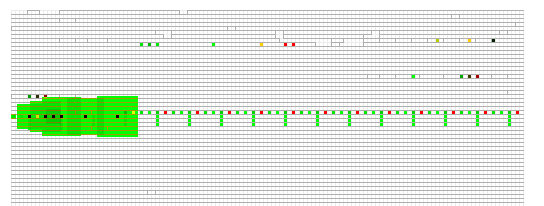
\includegraphics[scale=0.45]{images/example_haskell.png}
		\caption{Haskell example}
    \label{fig:example_array}
	\end{figure}

  For this example we inserted and read a set of integers into and from a haskell list, shown in figure \ref{fig:example_haskell}.
  
  Since we are language agnostic, we used the tool to inspect haskell code that performs the same operation. In this case there is a significant amount of startup accesses happening, which appear to initialize the haskell environment. A linear array still gets built, but bookkeeping happens at the beginning and end of every access. This display makes it very obvious where haskell incurs an overhead above the equivalent C++ implementation.
  
    % \begin{itemize}
    %   \item C++ array WITH STREAMING THROUGH
    %   \item C++ STL vector WITH PICTURE OF GROWTH AND REALLOC
    %   \item C++ STL map WITH PICTURE OF BINARY SEARCH
    %   \item Haskell list WITH PICTURE
    % \end{itemize}

\section{Related Work}\label{ch_r}

Visualizing Memory Graphs\cite{zimmerman:2001:VMG}, made the same observation that you want to drill down into memory structures, but they took a very different approach: they care about structures being built rather than than access to these structures. While we find this to be a useful inspection for debugging purposes, it does not directly show performance. It's a great example of memory visualization for debugging rather than performance.

KCacheGrind allows you to visualize the static structure of your code - similar to our stack traces - and also attaches performance events to it. While we take a very visual approach to this, KCacheGrind bubbles up statistics directly related to cache performance. This is useful for identifying issues, but we claim that our approach gives a direct visualization of the reasons behind the cache performance.

\section{Future Work}\label{ch_f}

  Future work for this project could proceed in two complementary directions:
    one in which we explore new methods for visualizing and interacting with data,
    and another in which we explore new methods for data collection and analysis.

  \subsection{Visualization and Interaction}
  %\begin{itemize}
  %  \item Diffmaps for comparing across revisions
  %  \item Aggregate views for massive amounts of data
  %  \item User-defined data filtering
  %  \item Bookmarking, Auto-Bookmarking
  %\end{itemize}

  Comparing alternative implementations of the same program is a difficult problem.
  Even a small change in access patterns or choice of data structures can render two traces nearly unrelatable.
  This could be mitigated somewhat by exploring techniques for canoncalizing memory event streams and identifying patterns
    that are invariant between two streams.
  Another complication worth exploring is prohibitively large memory event streams.  
  Future work could examine techniques for aggregating more data into a smaller part of the memory map,
    user-defined methods for filtering data based on events of interest,
    and tools for bookmarking those events either manually or automatically.

  \subsection{Data Collection and Analysis}
  %\begin{itemize}
  %  \item Physical memory simulator
  %  \item Supporting incomplete data / sampling
  %  \item Selective data capture
  %\end{itemize}

  PerVERT currently visualizes a program's use of the virtual address space, but says nothing about physical memory.
  However because performance is truly a function of physical memory usage, it would be useful to visualize that space as well.
  One way of doing so without being invasive would be to build in a cache simulator.
  Other areas that could be improved include support for analyzing incomplete data, 
    or for intelligently sampling from prohibitively large memory event traces.

\section{Conclusion}

In this paper we presented PerVERT, an instrumentation framework for logging a process's virtual memory traffic and 
  a visualization suite for reasoning about common memory performance bugs.
We described the design goals that lead us to its current form,
  and through several small prototypical examples, demonstrated the effectiveness of its current design.
In its current state, PerVERT functions well as a final class project.
However, it is our intention to continue development as described above, and to evolve its design into a mature research tool.

\bibliographystyle{acmsiggraph}
\bibliography{template}
\end{document}
